% =============================================================================
% Re-evaluating Re-rankers: A Methodological Critique of Calibration on
% Retrieval Benchmarks   --   FIRE conference track (ACM acmart / sigconf)
%
% Compile: tectonic calrank_fire.tex   (fetches acmart automatically)
% Target length: up to 8 pages. Limitations are added separately by the authors.
%
% For camera-ready: remove [nonacm], add the FIRE rights block, \acmConference,
% year, DOI, and the CCS concepts block from the ACM classification tool.
% =============================================================================
\documentclass[sigconf,nonacm]{acmart}

\usepackage{booktabs}
\usepackage{colortbl}   % \rowcolor; acmart already loads xcolor
\usepackage{enumitem}
\usepackage{amsmath}
\usepackage{balance}

\definecolor{headblue}{HTML}{2C3E6B}
\definecolor{rowlight}{HTML}{EAF0FA}
\definecolor{cleangreen}{HTML}{E6F5E8}
\definecolor{singleclasspink}{HTML}{FDE8E8}
\definecolor{bestcell}{HTML}{D5F5E3}
\newcommand{\thead}[1]{\textbf{#1}}
\newcommand{\ece}{\mathrm{ECE}}
\newcommand{\sig}{\sigma}

\graphicspath{{../data/figures/}}
\emergencystretch=1.5em   % absorb minor overfull lines

\settopmatter{printacmref=false}
\renewcommand\footnotetextcopyrightpermission[1]{}
\pagestyle{plain}

\begin{document}

\title{Re-evaluating Re-rankers: A Methodological Critique of Calibration on
Retrieval Benchmarks}

\author{Sayanjib Sur}
\orcid{0009-0002-7967-2063}
\affiliation{%
  \institution{Department of Information Technology, Jadavpur University}
  \city{Kolkata}
  \country{India}}
\email{work.sayanjib@gmail.com}

\author{Pawan Kumar Singh}
\orcid{0000-0002-9598-7981}
\affiliation{%
  \institution{Department of Information Technology, Jadavpur University}
  \city{Kolkata}
  \country{India}}
\email{pawansingh.ju@gmail.com}

% =============================================================================
\begin{abstract}
The relevance scores produced by cross-encoder re-rankers are increasingly consumed
as probabilities: retrieval-augmented generation pipelines threshold on them,
abstention layers gate on them, and cascades route on them. Whether those scores are
calibrated has not been examined systematically, and a large part of the reason,
we argue, is that the benchmarks themselves cannot measure it. We conduct a
cross-domain calibration study of seven cross-encoder re-rankers over eleven
collections and use it to expose a methodological hazard: because most standard
retrieval collections are annotated by marking relevant documents and leaving the
rest unjudged, their judged sets contain few or no negatives, and on such data
calibration evaluation degenerates. A calibrator that maps every input to the
majority class attains a perfect score, so a naive pooled analysis reports that
isotonic regression is near-flawless and temperature scaling unreliable, and both
conclusions are wrong. We contribute a pre-flight validity diagnostic that flags
affected collections in advance; fixed before inspecting any result, it excludes six
of eleven collections, including one whose degeneracy is invisible to a prevalence
threshold and is independently confirmed by two further symptoms. Acting on the
diagnostic, we adopt the deeply pooled TREC Deep Learning collections. On the five
collections that pass, all three post-hoc corrections reduce calibration error
significantly (every pairwise comparison survives Holm--Bonferroni correction), they
leave ranking quality untouched to within $10^{-4}$ nDCG@10, and they convert a
threshold that delivered anywhere from $36\%$ to $85\%$ precision at a nominal cut of
$0.8$ into one that delivers $79\%$ to $87\%$. We package the corrections as a
per-model deployment recipe and release all scored pairs, fitted calibrators, and
code.
\end{abstract}

\keywords{calibration, cross-encoder re-ranking, retrieval evaluation, expected
calibration error, incomplete judgments, BEIR, TREC Deep Learning,
retrieval-augmented generation}

\maketitle

% =============================================================================
\section{Introduction}\label{sec:intro}

A cross-encoder re-ranker reads a query and a candidate document jointly and emits a
scalar relevance score; sorting by that score is the second stage of the standard
two-stage retrieval pipeline~\cite{nogueira2019}. What is newer is the practice of
reading the score not as a sorting key but as a probability. Retrieval-augmented
generation forwards only passages scoring above a fixed threshold~\cite{lewis2020rag};
abstention layers decline to answer when no candidate is confident enough; cascades
route low-confidence queries to larger models~\cite{gao2024rag}. Each treats
$\sig(\text{logit})$ as $P(\text{relevant} \mid q, d)$.

That interpretation is not licensed by training. Re-rankers are optimised for correct
ordering, and ordering competence does not entail probabilistic
accuracy~\cite{degroot1983,guo2017}: a model can rank flawlessly while assigning
probabilities that are systematically wrong. Whether re-ranker scores are calibrated
is therefore an open empirical question. Calibration has been studied for image
classifiers~\cite{guo2017,minderer2021} and language
models~\cite{kadavath2022,geng2024survey}, and touched for neural ranking in narrow
settings~\cite{penha2021,cohen2021}, but no systematic cross-domain account of
cross-encoder re-rankers exists.

We provide one, and in doing so make a claim that is as much about the benchmarks as
about the models: \emph{the standard retrieval collections used to evaluate ranking
cannot, for the most part, measure calibration}. The reason is structural.
Collections such as those in BEIR~\cite{thakur2021beir} are annotated by pooling and
judging candidate documents, and unjudged documents are treated as absent rather than
as non-relevant. The judged set is consequently dominated by, or composed entirely
of, positive labels. On such data the quantity that calibration metrics estimate is
degenerate: a constant predictor is perfectly calibrated, and the comparison between
calibration methods inverts. An analyst following standard practice would conclude
that the trivial method is best and a sound method unreliable.

This methodological critique is the paper's primary contribution; the calibration
study is the vehicle that exposes it and the setting in which we then show how to
proceed correctly. Concretely:

\begin{itemize}[leftmargin=1.2em,itemsep=2pt]
  \item We conduct the first systematic calibration study of cross-encoder
  re-rankers: seven models ($4$M--$560$M parameters) over eleven collections, with
  ECE, MCE, and Brier score and query-level bootstrap intervals
  (Section~\ref{sec:overconf}).
  \item We identify and explain the judgment-structure hazard, and distinguish it
  from the classical incomplete-judgments problem, which it survives
  (Section~\ref{sec:hazard}).
  \item We contribute a pre-flight validity diagnostic, fixed a priori, that flags
  affected collections and is corroborated by two independent symptoms; acting on it,
  we adopt the deeply pooled TREC Deep Learning collections
  (Section~\ref{sec:diagnostic}).
  \item On collections that pass, we establish a significant, ranking-preserving
  improvement, package it as a per-model deployment recipe, and show that its
  practical value is a threshold that means what it says
  (Sections~\ref{sec:valid}--\ref{sec:consequences}).
\end{itemize}

All artifacts are released.\footnote{\url{https://github.com/Codewithsayanjib/CalRank}}

% =============================================================================
\section{Background and Related Work}\label{sec:related}

\subsection{Cross-encoder re-ranking}
The two-stage pipeline pairs a fast first-stage retriever, classically
BM25~\cite{robertson2009bm25}, with a neural re-ranker that reads each query--document
pair jointly~\cite{nogueira2019}. The joint encoding is what distinguishes
cross-encoders from bi-encoders~\cite{reimers2019sbert}, which embed query and
document separately and interact only through a similarity function; by attending
across both inputs at once, cross-encoders model token-level interactions at higher
inference cost, which is why they sit in the second stage. Compact distilled variants
such as MiniLM~\cite{wang2020minilm} and TinyBERT~\cite{jiao2020tinybert}, and models
such as ELECTRA~\cite{clark2020electra} and BGE~\cite{xiao2023bge}, all emit a single
logit mapped through a sigmoid, and that value is what downstream systems consume.

\subsection{Measuring calibration}
A predictor is calibrated when its confidence matches empirical
accuracy~\cite{degroot1983}: of all predictions made with confidence $0.8$, about
$80\%$ should be correct. Expected Calibration Error~\cite{naeini2015} makes this
concrete by partitioning predictions into $B$ bins and averaging the per-bin gap
between confidence and accuracy, weighted by bin population:
\begin{equation}
\ece = \sum_{b=1}^{B} \frac{n_b}{N}\,\bigl|\,\mathrm{acc}(b) - \mathrm{conf}(b)\,\bigr|.
\end{equation}
ECE is the most reported calibration metric, though it is sensitive to the binning
scheme~\cite{nixon2019,roelofs2022}; we fix fifteen equal-width bins throughout and
verify the choice does not drive the results. Maximum Calibration Error reports the
single worst bin, and the Brier score~\cite{brier1950}, the mean squared error between
predicted probability and outcome, is a proper scoring rule that rewards calibration
and discrimination jointly. Reliability diagrams~\cite{niculescu2005} plot accuracy
against confidence; a calibrated model traces the diagonal, and bars below it signal
overconfidence.

\subsection{Post-hoc correction}
Calibration can be corrected after training, without touching the model, by fitting a
small transform on held-out data. \emph{Temperature scaling}~\cite{guo2017} divides
the logit by a learned scalar $T$, $p = \sig(z/T)$; for $T>1$ it softens
overconfidence. \emph{Platt scaling}~\cite{platt1999} fits a two-parameter logistic
regression $p = \sig(az+b)$; the intercept $b$ lets it shift the operating point that
temperature cannot move. \emph{Isotonic regression}~\cite{zadrozny2002} fits a
non-parametric monotone step function, the most flexible option and the most prone to
overfitting on small sets. Crucially, all three are \emph{monotone}: they never
reorder documents, so they cannot harm ranking quality, a property we exploit in
Section~\ref{sec:consequences}. Beyond these, Dirichlet
calibration~\cite{kull2019} extends the parametric family to the multiclass case; the
binary relevance decision here is well served by the three classical methods.
Calibration has been revisited for modern classifiers~\cite{minderer2021} and studied
for LLMs~\cite{kadavath2022,tian2023,geng2024survey} and NLI~\cite{desai2020}, and the
selective-prediction literature~\cite{geifman2017,el2010} depends on calibrated
confidence, though rarely makes the dependence explicit for retrieval.

\subsection{Calibration in ranking, and incomplete judgments}
Closest to us, Penha and Hauff~\cite{penha2021} examine calibration and uncertainty in
neural learning-to-rank; their setting is conversational response ranking, where
negatives are a design parameter of the task, whereas ours is cross-domain retrieval
over collections whose judgment structure is inherited from pooling---the very
property that produces the hazard studied here, and which their setting does not
exhibit. Cohen et al.~\cite{cohen2021} study uncertainty for ranking through a
Bayesian lens. Separately, that test collections are incompletely judged is long
established~\cite{buckley2004,lu2016}, with remedies including bpref~\cite{buckley2004},
inferred measures~\cite{yilmaz2006}, and condensed-list evaluation~\cite{sakai2007}.
That literature concerns \emph{unjudged} documents biasing ranking metrics, and its
remedy is to evaluate on judged documents only. As Section~\ref{sec:hazard} shows,
our hazard is distinct: it arises \emph{within} the judged set, survives judged-only
evaluation, and inverts a method comparison rather than biasing a metric value.

% =============================================================================
\section{Experimental Setup}\label{sec:setup}

\paragraph{Models.}
Seven publicly available cross-encoders spanning $4$M to $560$M parameters
(Table~\ref{tab:models}). The first five are MS~MARCO-trained and form the main set;
two (mxbai-base, BGE-large) were added to widen scale and training data. All
checkpoints are drawn unmodified from the Hugging Face Hub.\footnote{Model pages at \url{https://huggingface.co/}$\langle$id$\rangle$ for the identifiers in Table~\ref{tab:models}.} MiniLM-L6 and MiniLM-L12 are the default re-rankers in LangChain, LlamaIndex, and Haystack,\footnote{\url{https://python.langchain.com}, \url{https://www.llamaindex.ai}, \url{https://haystack.deepset.ai}.} so the population is not hypothetical but the models practitioners actually deploy.

\begin{table}[t]
\centering
\caption{The seven cross-encoder re-rankers. Identifiers under the
\texttt{cross-encoder/} namespace are shown without that prefix. $\dagger$ marks the
two added to widen scale and training data; mxbai-base is not MS~MARCO-trained.}\label{tab:models}
\footnotesize
\setlength{\tabcolsep}{4pt}
\begin{tabular}{llr}
\toprule
\thead{Model} & \thead{HuggingFace identifier} & \thead{Params} \\
\midrule
TinyBERT-L2~\cite{jiao2020tinybert}  & ms-marco-TinyBERT-L-2-v2 & 4M \\
MiniLM-L6~\cite{wang2020minilm}    & ms-marco-MiniLM-L-6-v2   & 22M \\
MiniLM-L12~\cite{wang2020minilm}   & ms-marco-MiniLM-L-12-v2  & 33M \\
ELECTRA-base~\cite{clark2020electra} & ms-marco-electra-base  & 110M \\
mxbai-base$^{\dagger}$   & mixedbread-ai/mxbai-rerank-base-v1 & 184M \\
BGE-base~\cite{xiao2023bge}     & BAAI/bge-reranker-base       & 278M \\
BGE-large$^{\dagger}$~\cite{xiao2023bge}    & BAAI/bge-reranker-large & 560M \\
\bottomrule
\end{tabular}
\end{table}

\paragraph{Collections.}
Nine BEIR collections~\cite{thakur2021beir} and the two TREC Deep Learning passage
collections~\cite{craswell2020}, ordered by prevalence in
Table~\ref{tab:collections}.\footnote{BEIR: \url{https://github.com/beir-cellar/beir}; TREC~DL judgments and pools: \url{https://microsoft.github.io/msmarco/TREC-Deep-Learning}.} Prevalence, the fraction of judged pairs that are positive, is the property this paper turns on.

\begin{table}[t]
\centering
\caption{The eleven collections, ordered by prevalence.
\textcolor{green!50!black}{Green} passes the validity diagnostic of
Section~\ref{sec:diagnostic}; \textcolor{red!50!black}{pink} fails.}
\label{tab:collections}
\small
\begin{tabular}{lrrrl}
\toprule
\thead{Collection} & \thead{Judged} & \thead{Prev.} & \thead{Neg.} & \thead{Domain} \\
\midrule
\rowcolor{cleangreen}
trec-dl-2020     & 5{,}686 & 0.17 & 4{,}727 & web passages \\
\rowcolor{cleangreen}
dbpedia-entity   & 9{,}182 & 0.35 & 5{,}996 & entity \\
\rowcolor{cleangreen}
trec-dl-2019     & 4{,}612 & 0.35 & 3{,}000 & web passages \\
\rowcolor{cleangreen}
trec-covid       & 3{,}475 & 0.62 & 1{,}306 & biomedical \\
\rowcolor{cleangreen}
webis-touche2020 & 635     & 0.78 & 140     & argument \\
\rowcolor{singleclasspink}
scidocs          & 1{,}774 & 0.95 & 91      & citation \\
\rowcolor{singleclasspink}
arguana          & 1{,}316 & 1.00 & 0       & counter-arg. \\
\rowcolor{singleclasspink}
fiqa             & 756     & 1.00 & 0       & financial QA \\
\rowcolor{singleclasspink}
nfcorpus         & 1{,}941 & 1.00 & 0       & health \\
\rowcolor{singleclasspink}
quora            & 1{,}278 & 1.00 & 0       & duplicates \\
\rowcolor{singleclasspink}
scifact          & 298     & 1.00 & 0       & claims \\
\bottomrule
\end{tabular}
\end{table}

\paragraph{Pipeline.}
For each query we retrieve the BM25 top~100 with \texttt{bm25s}\footnote{\url{https://github.com/xhluca/bm25s}} ($k_1{=}0.9$, $b{=}0.4$) and score every pair with every model via \texttt{sentence-transformers}~\cite{reimers2019sbert}, storing the raw logit, its sigmoid, and the
binarised judgment ($-1$ unjudged, $0$ judged non-relevant, $1$ judged relevant). For
the TREC~DL collections, whose official top-1000 pool is not rank-ordered, we score
every judged pair in the pool. This yields roughly half a million scored pairs, about
twenty thousand judged per model. All computation ran on a single Apple~M4; the study
reproduces on a laptop, and every analysis below is a re-analysis of stored logits
requiring no further inference. Calibrators and statistics use \texttt{scikit-learn} and \texttt{SciPy}.\footnote{\url{https://scikit-learn.org}, \url{https://scipy.org}.}

\paragraph{Metrics and protocol.}
ECE, MCE, and Brier score use fifteen equal-width bins, with a $95\%$ confidence
interval on ECE from a query-level bootstrap of $1{,}000$ resamples (query-level
because judgments within a query are dependent). For each model--collection pair we
split judged pairs $50/50$, stratified by label, seed $42$; calibrators are fitted on
one half and evaluated on the other, so no calibrator is ever scored on the data it
was fitted to. Held-out evaluation matters most for isotonic regression, which can
otherwise reproduce its fitting distribution and report an implausibly low error.

% =============================================================================
\section{Re-rankers Are Overconfident}\label{sec:overconf}

On the five collections that pass the diagnostic, across the five main models
($25$ pairs), mean raw ECE is $0.280$ and optimal temperatures range from about three
to twelve: the raw sigmoid is not a usable probability. Figure~\ref{fig:heatmap}
shows the pattern across all pairs, and Table~\ref{tab:permodel} summarises it per
model. A signed, bin-weighted ECE confirms overconfidence in $20$ of $25$ pairs
(mean $+0.139$); the clearest cases are the low-prevalence collections, most severely
trec-dl-2020 ($+0.294$ at prevalence $0.17$), consistent with models trained on
MS~MARCO, where almost every candidate is relevant, carrying a prior that is too high
for collections where most candidates are not.

\begin{figure}[t]
\centering
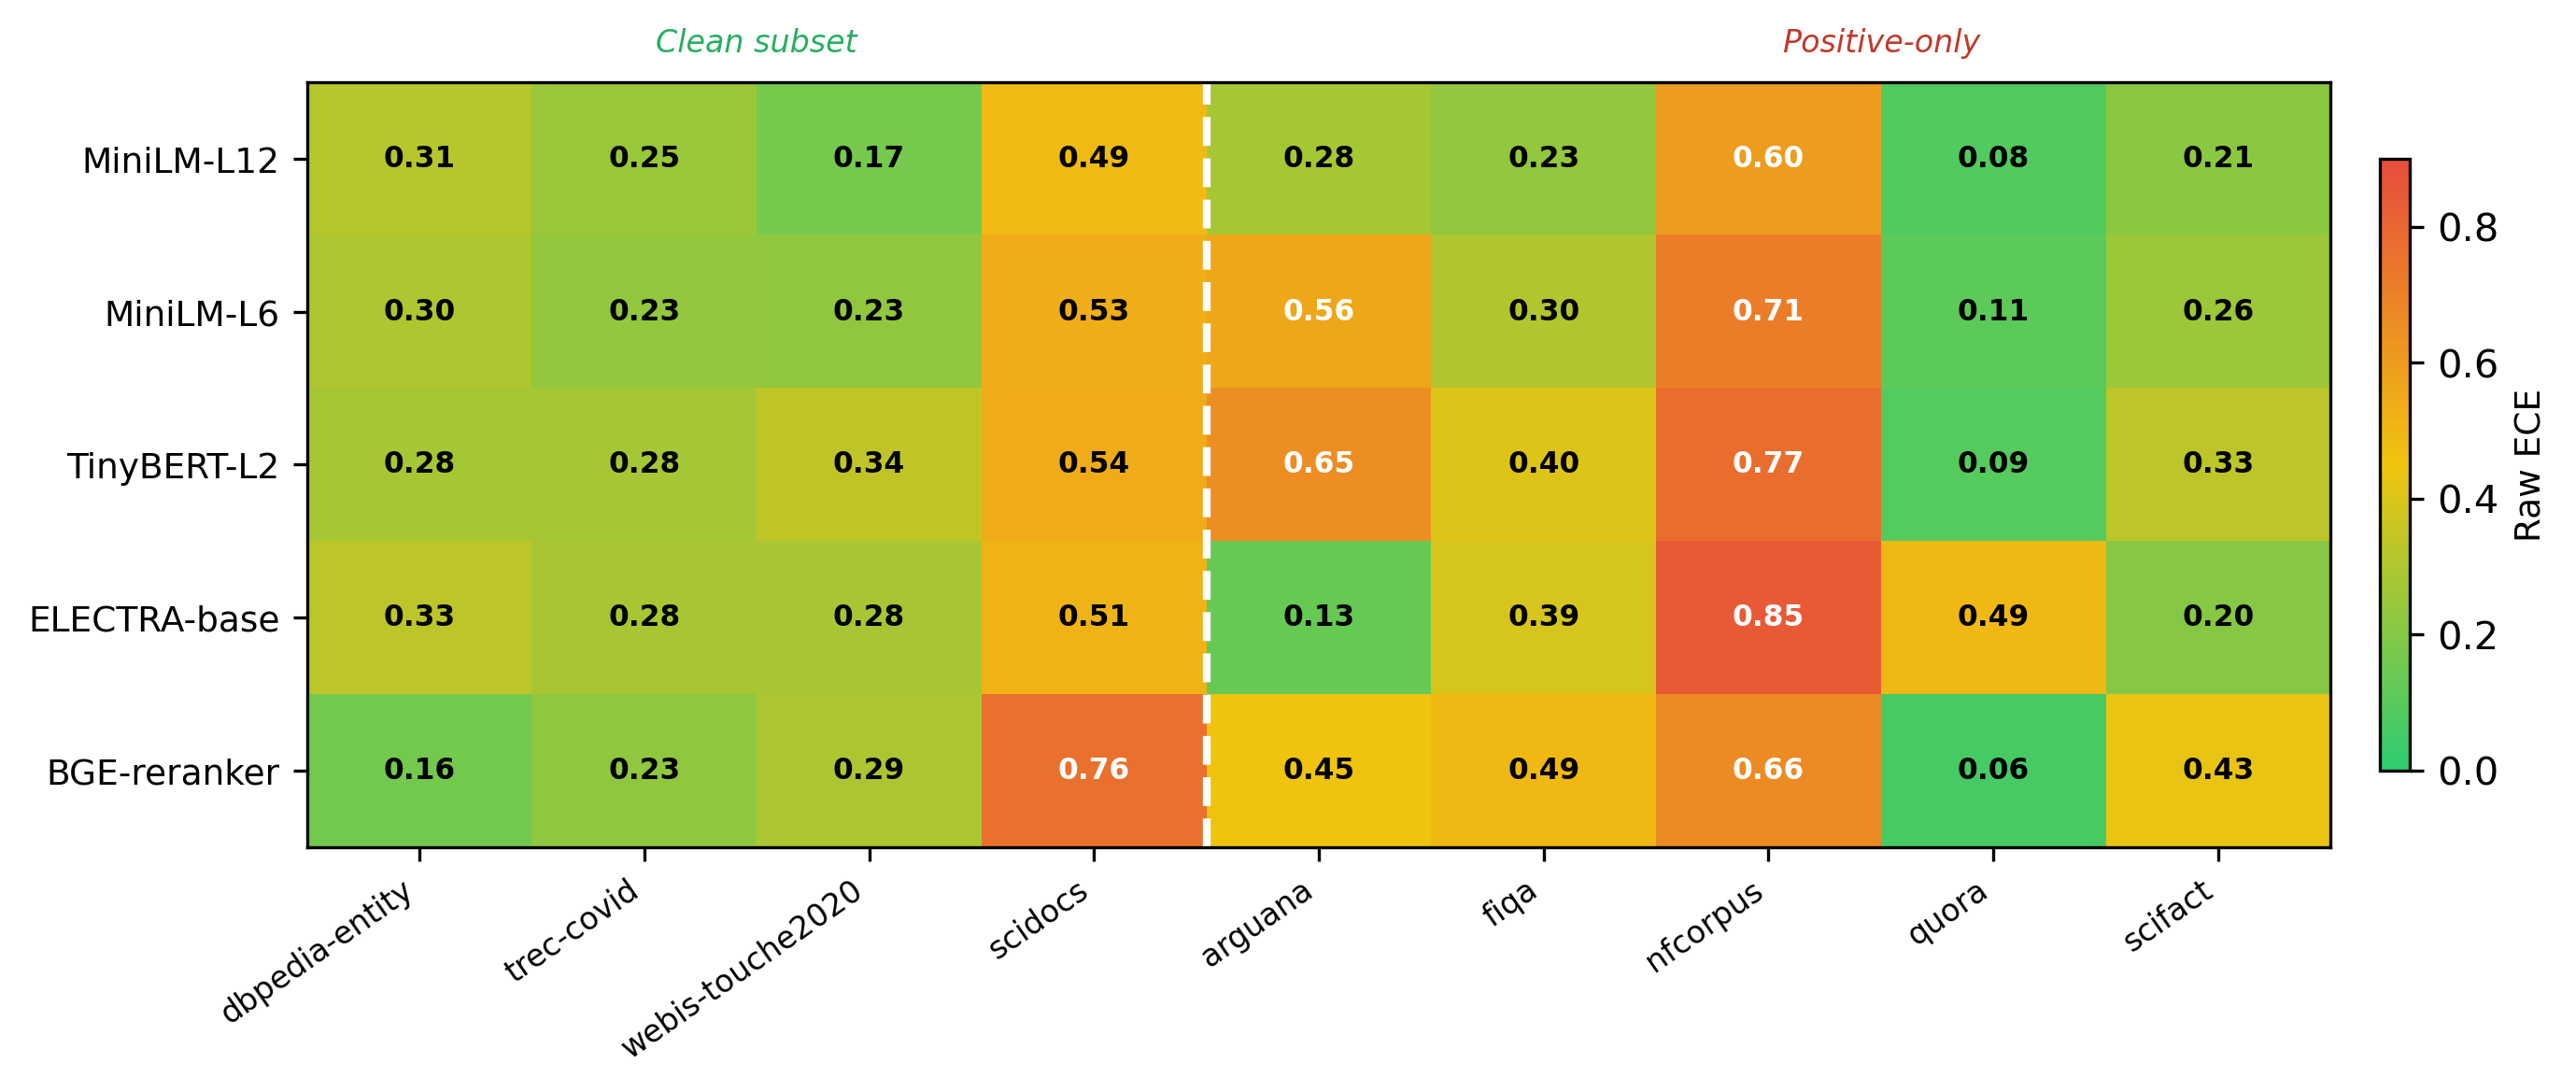
\includegraphics[width=\columnwidth]{paper_fig_ece_heatmap.png}
\Description{Heatmap of raw expected calibration error for seven re-rankers across eleven collections. Most cells are warm-coloured, indicating high error; the positive-only collections on the right are uniformly poor.}
\caption{Raw ECE across all model--collection pairs. Green is low error, red high; the
dashed line separates the collections that pass the diagnostic (left) from those that
fail (right).}\label{fig:heatmap}
\end{figure}

\begin{table}[t]
\centering
\caption{Per-model summary on the valid subset. $T$ is the mean optimal temperature.
Every model needs substantial softening; the two most recent models ($\dagger$) need
the least.}\label{tab:permodel}
\small
\begin{tabular}{lrrrr}
\toprule
\thead{Model} & \thead{Params} & \thead{mean $T$} & \thead{raw ECE} & \thead{temp ECE} \\
\midrule
TinyBERT-L2  & 4M   & 8.69 & 0.323 & 0.202 \\
MiniLM-L6    & 22M  & 6.24 & 0.295 & 0.202 \\
MiniLM-L12   & 33M  & 6.84 & 0.296 & 0.197 \\
ELECTRA-base & 110M & 5.29 & 0.257 & 0.124 \\
mxbai-base$^{\dagger}$   & 184M & 1.99 & \textbf{0.136} & 0.123 \\
BGE-base     & 278M & 4.16 & 0.230 & 0.162 \\
BGE-large$^{\dagger}$    & 560M & 3.49 & 0.202 & 0.120 \\
\bottomrule
\end{tabular}
\end{table}

% =============================================================================
\section{The Hazard: Benchmarks That Cannot Measure Calibration}\label{sec:hazard}

This is the core of the critique. Six of the eleven collections have almost no
negative judgments; five have exactly none (Table~\ref{tab:collections}). On a
collection where every judged label is positive, calibration evaluation is degenerate:
a predictor that outputs $1.0$ for everything has confidence equal to accuracy and
attains $\ece = 0$. That is not calibration; it is a degenerate answer to a degenerate
question.

Isotonic regression realises exactly this. On single-class fitting splits it maps all
inputs to the majority class and scores $\ece = 0.000$ on the held-out split---a
figure that looks flawless only if its origin is unknown. Temperature scaling,
conversely, has no negative examples from which to learn a reduction in confidence;
its optimum diverges, collapsing every probability toward $0.5$, and it can
\emph{increase} ECE (Figure~\ref{fig:backfire}).

\begin{figure}[t]
\centering
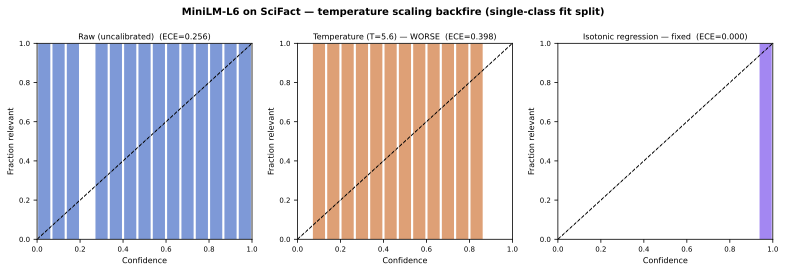
\includegraphics[width=0.82\columnwidth]{paper_fig2_minilm_scifact_temp_backfire.png}
\Description{Two reliability diagrams for MiniLM-L6 on the single-class scifact collection. Temperature scaling increases calibration error while isotonic regression collapses to a trivial zero.}
\caption{MiniLM-L6 on scifact (prevalence $1.0$): temperature scaling worsens ECE
while isotonic regression attains a trivial zero. Neither number reflects
calibration.}\label{fig:backfire}
\end{figure}

The consequence is not a biased number but an inverted conclusion. Pooling all $45$
model--collection pairs, temperature scaling appears to improve ECE in only $27$
(Wilcoxon $p{=}0.024$) while isotonic appears to improve all $45$. The natural
reading, that temperature is unreliable and isotonic excellent, is wrong in both
halves and is produced entirely by the degenerate collections.

\paragraph{Why this is not the incomplete-judgments problem.}
The classical concern is \emph{unjudged} documents biasing ranking metrics, and its
remedy is judged-only evaluation~\cite{buckley2004,sakai2007}. Our hazard survives
that remedy: we already evaluate on judged pairs only, and the degeneracy arises from
the class balance within the judged set. The mechanism differs (missing mass outside
the pool versus label imbalance inside it), and so does the effect: the established
problem depresses a metric value while leaving system comparisons roughly intact,
whereas ours inverts the comparison between calibration methods. A study could apply
every remedy in that literature and still choose the wrong calibrator, because those
remedies repair ranking metrics and are silent about probabilities.

% =============================================================================
\section{A Pre-flight Validity Diagnostic}\label{sec:diagnostic}

An observation is more useful as a check. We state one, fixed before inspecting any
calibration result: evaluation on a collection is valid only if
\begin{equation}
\min(n_+, n_-) \geq 100 \quad\text{and}\quad \pi \leq 0.90,
\end{equation}
where $n_+, n_-$ count positive and negative judged pairs and $\pi$ is prevalence. The
first condition guarantees enough minority support for the per-bin estimates ECE
aggregates; the second excludes collections so skewed that a constant predictor scores
near zero. Both thresholds are conventional and were not tuned.

Applied to all eleven collections, the diagnostic flags six. Five are the
positive-only collections. The sixth is informative: scidocs, at prevalence $0.95$
with only $91$ negatives, which we had initially treated as clean and which would
survive any prevalence-only criterion below $0.95$. Two independent symptoms,
established elsewhere without reference to the diagnostic, confirm it is degenerate:
its fitted temperature diverges under an uncapped search (behaviour otherwise confined
to positive-only collections), and it is the sole putatively-clean collection whose
calibrator-transfer behaviour departs from its neighbours
(Section~\ref{sec:consequences}). A criterion fixed a priori and two unrelated
empirical signatures converging on the same collection is strong evidence that the
criterion tracks something real.

Acting on the diagnostic, we adopt the deeply pooled TREC Deep Learning 2019 and 2020
passage collections, which supply $3{,}000$ and $4{,}727$ negatives---more than any
BEIR collection here---and pass comfortably. This takes the usable set from three
collections to five, and gives the study a base spanning prevalences from $0.17$ to
$0.78$.

% =============================================================================
\section{What Holds When Measurement Is Valid}\label{sec:valid}

On the five valid collections ($25$ pairs), every method improves ECE, in a consistent
order: raw $0.280 \to$ temperature $0.177 \to$ Platt $0.046 \to$ isotonic $0.029$
(Table~\ref{tab:valid}). Because six comparisons are drawn from the same data we apply
Holm--Bonferroni correction across the whole family; all six survive at
$\alpha{=}0.05$ with large effect sizes (Table~\ref{tab:stats}). A per-collection
breakdown is uniform: on each collection individually, every method beats the raw
baseline for every model.

\begin{table}[t]
\centering
\caption{Mean ECE by collection on the valid subset, ordered by prevalence. The
ordering isotonic $>$ Platt $>$ temperature holds throughout, and temperature's
deficit widens as prevalence departs from balance.}\label{tab:valid}
\small
\begin{tabular}{lrrrrr}
\toprule
\thead{Collection} & \thead{$\pi$} & \thead{raw} & \thead{temp} & \thead{Platt} & \thead{iso} \\
\midrule
trec-dl-2020     & 0.17 & 0.324 & 0.284 & 0.021 & 0.016 \\
dbpedia-entity   & 0.35 & 0.276 & 0.182 & 0.030 & 0.022 \\
trec-dl-2019     & 0.35 & 0.285 & 0.146 & 0.043 & 0.039 \\
trec-covid       & 0.62 & 0.255 & 0.056 & 0.054 & 0.031 \\
webis-touche2020 & 0.78 & 0.262 & 0.221 & 0.082 & 0.038 \\
\midrule
\rowcolor{bestcell}
\textbf{Mean}    &      & \textbf{0.280} & \textbf{0.177} & \textbf{0.046} & \textbf{0.029} \\
\bottomrule
\end{tabular}
\end{table}

\begin{table}[t]
\centering
\caption{Method comparisons with Holm--Bonferroni correction across the family of six
tests. Negative $\Delta$ favours the first-named method; all six are significant.}
\label{tab:stats}
\small
\begin{tabular}{lrrrc}
\toprule
\thead{Comparison} & \thead{mean $\Delta$} & \thead{$d_z$} & \thead{wins} & \thead{$p_{\text{Holm}}$} \\
\midrule
temp vs.\ raw       & $-0.108$ & $-1.37$ & 20/20 & $1.1{\times}10^{-5}$ \\
Platt vs.\ raw      & $-0.295$ & $-1.72$ & 20/20 & $1.1{\times}10^{-5}$ \\
iso vs.\ raw        & $-0.314$ & $-1.97$ & 20/20 & $1.1{\times}10^{-5}$ \\
Platt vs.\ temp     & $-0.187$ & $-1.08$ & 17/20 & $9.5{\times}10^{-5}$ \\
iso vs.\ temp       & $-0.206$ & $-1.26$ & 20/20 & $1.1{\times}10^{-5}$ \\
iso vs.\ Platt      & $-0.019$ & $-0.86$ & 18/20 & $1.1{\times}10^{-4}$ \\
\bottomrule
\end{tabular}
\end{table}

The intercept is visible in the prevalence dependence. Where prevalence is near
balance (trec-covid, $0.62$) temperature and Platt are indistinguishable ($0.056$ vs.\
$0.054$); where it is far from balance (trec-dl-2020, $0.17$) temperature reaches only
$0.284$ against Platt's $0.021$, a thirteen-fold difference.
Figure~\ref{fig:fourpanel} shows the progression on a single collection. Temperature
can only rescale; correcting a shifted operating point requires the intercept that
Platt and isotonic supply.

\begin{figure}[t]
\centering
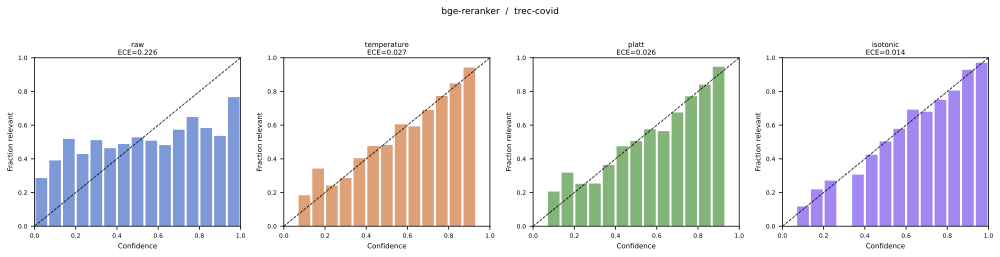
\includegraphics[width=0.98\columnwidth]{paper_fig_bge_treccovid_4panel.png}
\Description{Four reliability diagrams for BGE-base on trec-covid showing raw, temperature, Platt, and isotonic calibration. The bars move progressively from below the diagonal onto it.}
\caption{BGE-base on trec-covid: raw, temperature, Platt, isotonic. The reliability
bars move from well below the diagonal up onto it.}\label{fig:fourpanel}
\end{figure}

\paragraph{Model choice matters less than calibration.}
Raw ECE varies substantially across models, from $0.136$ for mxbai-base to $0.323$ for
TinyBERT-L2 (Table~\ref{tab:permodel}). Yet after Platt or isotonic correction all
seven models converge to within $0.014$ ECE. Selecting a better-calibrated re-ranker
and calibrating a worse one are close to substitutable, and since calibration is a
one-line change while swapping models means re-benchmarking the pipeline, calibrating
the model already in place is usually the cheaper route to the same place.

% =============================================================================
\section{Consequences for Deployment}\label{sec:consequences}

\subsection{Calibration is free}
Because all three methods are monotone, they cannot reorder documents. We confirm this
empirically: nDCG@10 changes by at most $1.0\times10^{-4}$ across all pairs
(Table~\ref{tab:downstream}). Calibration is obtained at no cost to ranking
effectiveness, which is what makes it safe to apply by default.

\begin{table}[t]
\centering
\caption{Ranking is untouched by calibration. Mean over models on the valid BEIR
collections; nDCG@10 and the accept rate at $p{>}0.5$ are identical before and after
correction.}\label{tab:downstream}
\small
\begin{tabular}{lrrrr}
\toprule
\thead{Collection} & \thead{nDCG@10} & \thead{MAP} & \thead{Acc.\ raw} & \thead{Acc.\ cal} \\
\midrule
dbpedia-entity   & 0.349 & 0.455 & 0.963 & 0.963 \\
trec-covid       & 0.686 & 0.680 & 0.988 & 0.988 \\
webis-touche2020 & 0.265 & 0.287 & 0.988 & 0.988 \\
\bottomrule
\end{tabular}
\end{table}

\subsection{A deployment recipe}
For a practitioner consuming re-ranker scores as probabilities, the immediate remedy
is a single scalar per model. Table~\ref{tab:recipe} reports the recommended
temperature, the mean optimum over the valid subset; dividing the logit by it before
the sigmoid is a one-line change that requires no retraining and substantially
improves calibration. Where a held-out set with genuine negatives is available from
the target domain, Platt scaling or isotonic regression improves further, and these
temperatures are a floor rather than a ceiling.

\begin{table}[t]
\centering
\caption{Deployment recipe: recommended per-model temperature (mean optimum on the
valid subset). Apply by dividing the logit by $T$ before the sigmoid.}\label{tab:recipe}
\small
\setlength{\tabcolsep}{4.5pt}
\begin{tabular}{lrrr}
\toprule
\thead{Model} & \thead{Params} & \thead{Rec.\ $T$} & \thead{ECE (raw$\to$temp)} \\
\midrule
mxbai-base   & 184M & 1.99 & 0.136 $\to$ 0.123 \\
BGE-large    & 560M & 3.49 & 0.202 $\to$ 0.120 \\
BGE-base     & 278M & 4.16 & 0.230 $\to$ 0.162 \\
ELECTRA-base & 110M & 5.29 & 0.257 $\to$ 0.124 \\
MiniLM-L6    & 22M  & 6.24 & 0.295 $\to$ 0.202 \\
MiniLM-L12   & 33M  & 6.84 & 0.296 $\to$ 0.197 \\
TinyBERT-L2  & 4M   & 8.69 & 0.323 $\to$ 0.202 \\
\bottomrule
\end{tabular}
\end{table}

\subsection{Temperature travels; the recipe is portable}
A per-model temperature is only useful as a recipe if it works on a domain it was not
fitted to. It does. Under leave-one-domain-out transfer (fit on four collections,
evaluate on the fifth), temperature retains $87\%$ of its in-domain benefit and beats
the raw scores in $22$ of $25$ cases (Figure~\ref{fig:transfer}), and the fitted
temperatures vary by only a factor of $1.7$ to $2.9$ across collections. This
stability is what licenses quoting one temperature per model. Platt scaling, whose
intercept encodes a domain-specific operating point, transfers less readily, so where
no in-domain data exists temperature is the recommended default.

\begin{figure}[t]
\centering
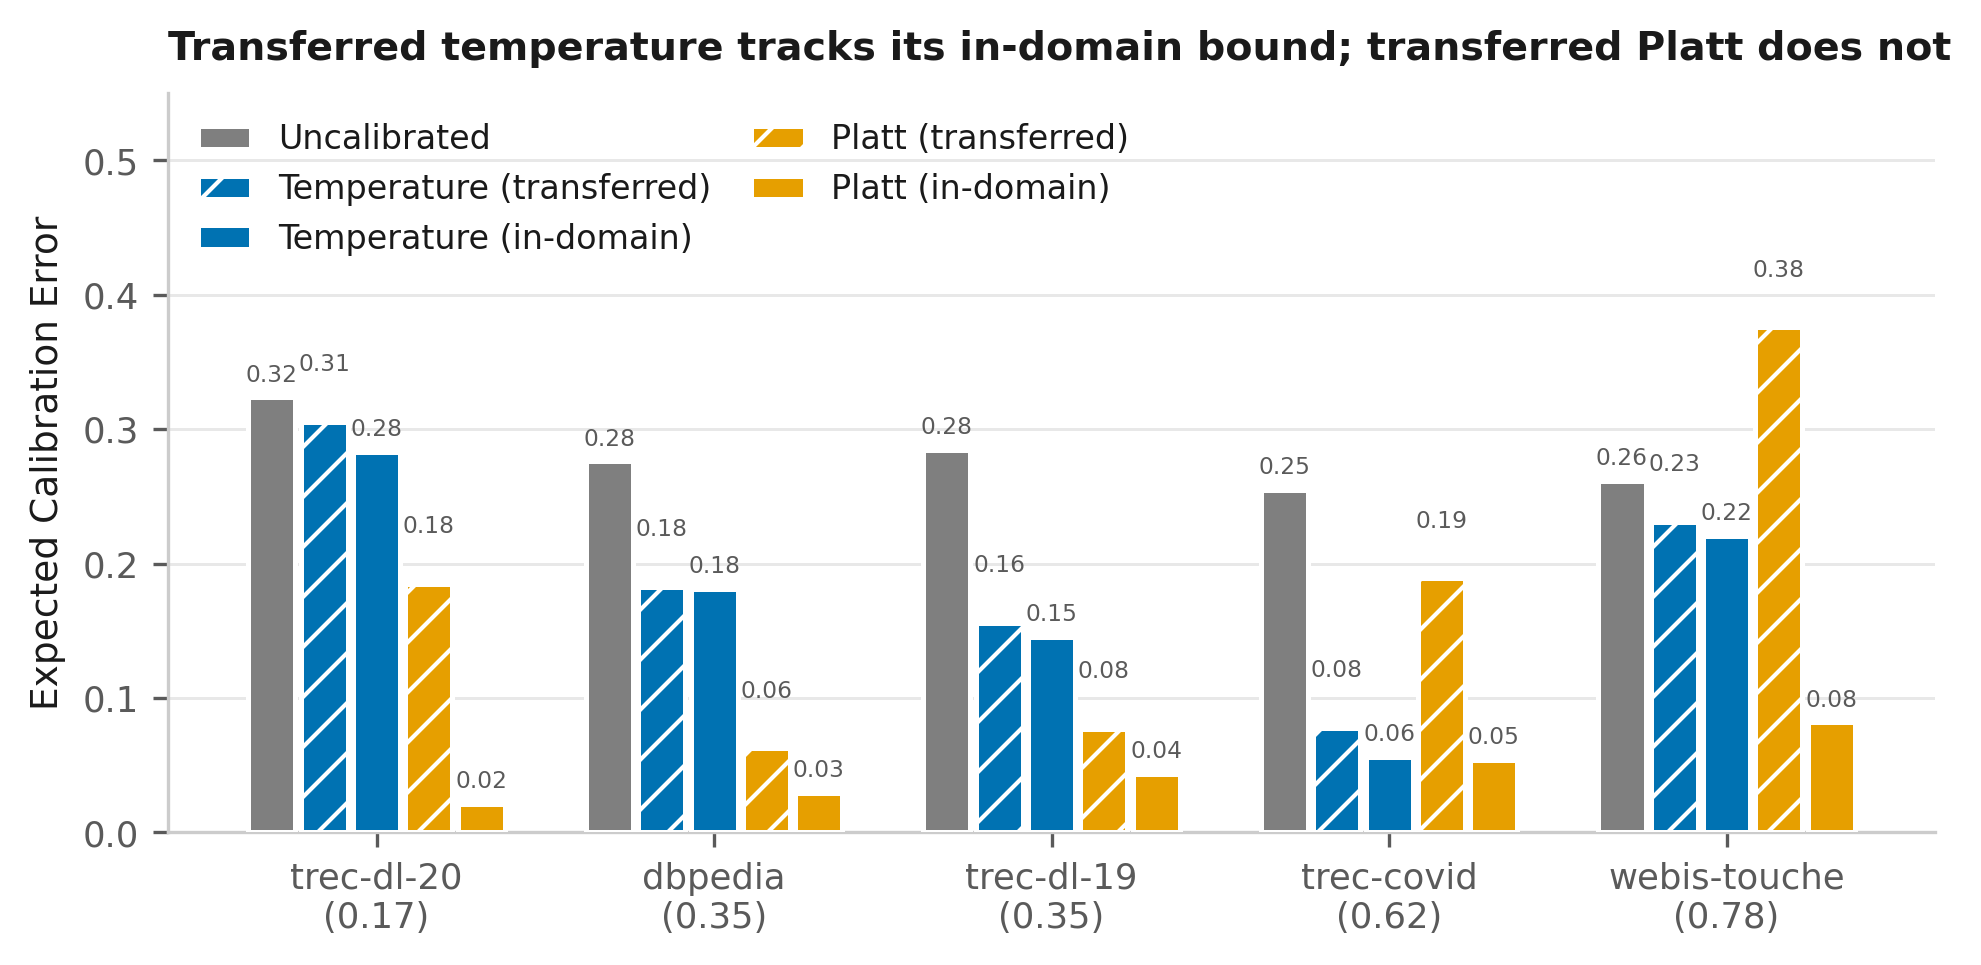
\includegraphics[width=\columnwidth]{paper_fig_transfer.png}
\Description{Grouped bar chart of expected calibration error under transferred and in-domain calibrators across five collections. Temperature bars are nearly equal in height across the two regimes; Platt bars differ substantially.}
\caption{Calibrator transfer on the valid subset. Hatched bars are transferred
(leave-one-domain-out) calibrators; solid bars are in-domain. Temperature (blue) is
nearly unchanged by transfer.}\label{fig:transfer}
\end{figure}

\subsection{What calibration buys: an honest threshold}
The monotonicity that makes calibration free also delimits what it does: it cannot
change the precision--coverage frontier, so it does not make a selective system better
at selecting. What it does is make a stated threshold mean what it says. Setting a cut
of $\tau = 0.8$, the realised precision uncalibrated ranges from $0.357$ on
trec-dl-2020 to $0.854$ on webis-touche2020---a spread of $0.497$, with the worst
collection delivering less than half the requested precision. After isotonic
calibration the range narrows to $0.789$--$0.867$, a spread of $0.078$
(Table~\ref{tab:threshold}, Figure~\ref{fig:honesty}). The same nominal setting, which
denoted five different operating points, now denotes approximately one. For any system
that gates on a confidence value, this portability is the practical payoff.

\begin{table}[t]
\centering
\caption{Realised precision when the operator requests $\tau{=}0.8$. Calibration
collapses the cross-collection spread from $0.497$ to $0.078$.}\label{tab:threshold}
\small
\begin{tabular}{lrrr}
\toprule
\thead{Collection} & \thead{Uncalib.} & \thead{Temp.} & \thead{Isotonic} \\
\midrule
trec-dl-2020     & 0.357 & 0.646 & 0.812 \\
dbpedia-entity   & 0.542 & 0.890 & 0.867 \\
trec-dl-2019     & 0.553 & 0.765 & 0.789 \\
trec-covid       & 0.712 & 0.843 & 0.844 \\
webis-touche2020 & 0.854 & 0.783 & 0.851 \\
\midrule
\rowcolor{bestcell}
\textbf{Spread}  & \textbf{0.497} & 0.243 & \textbf{0.078} \\
\bottomrule
\end{tabular}
\end{table}

\begin{figure}[t]
\centering
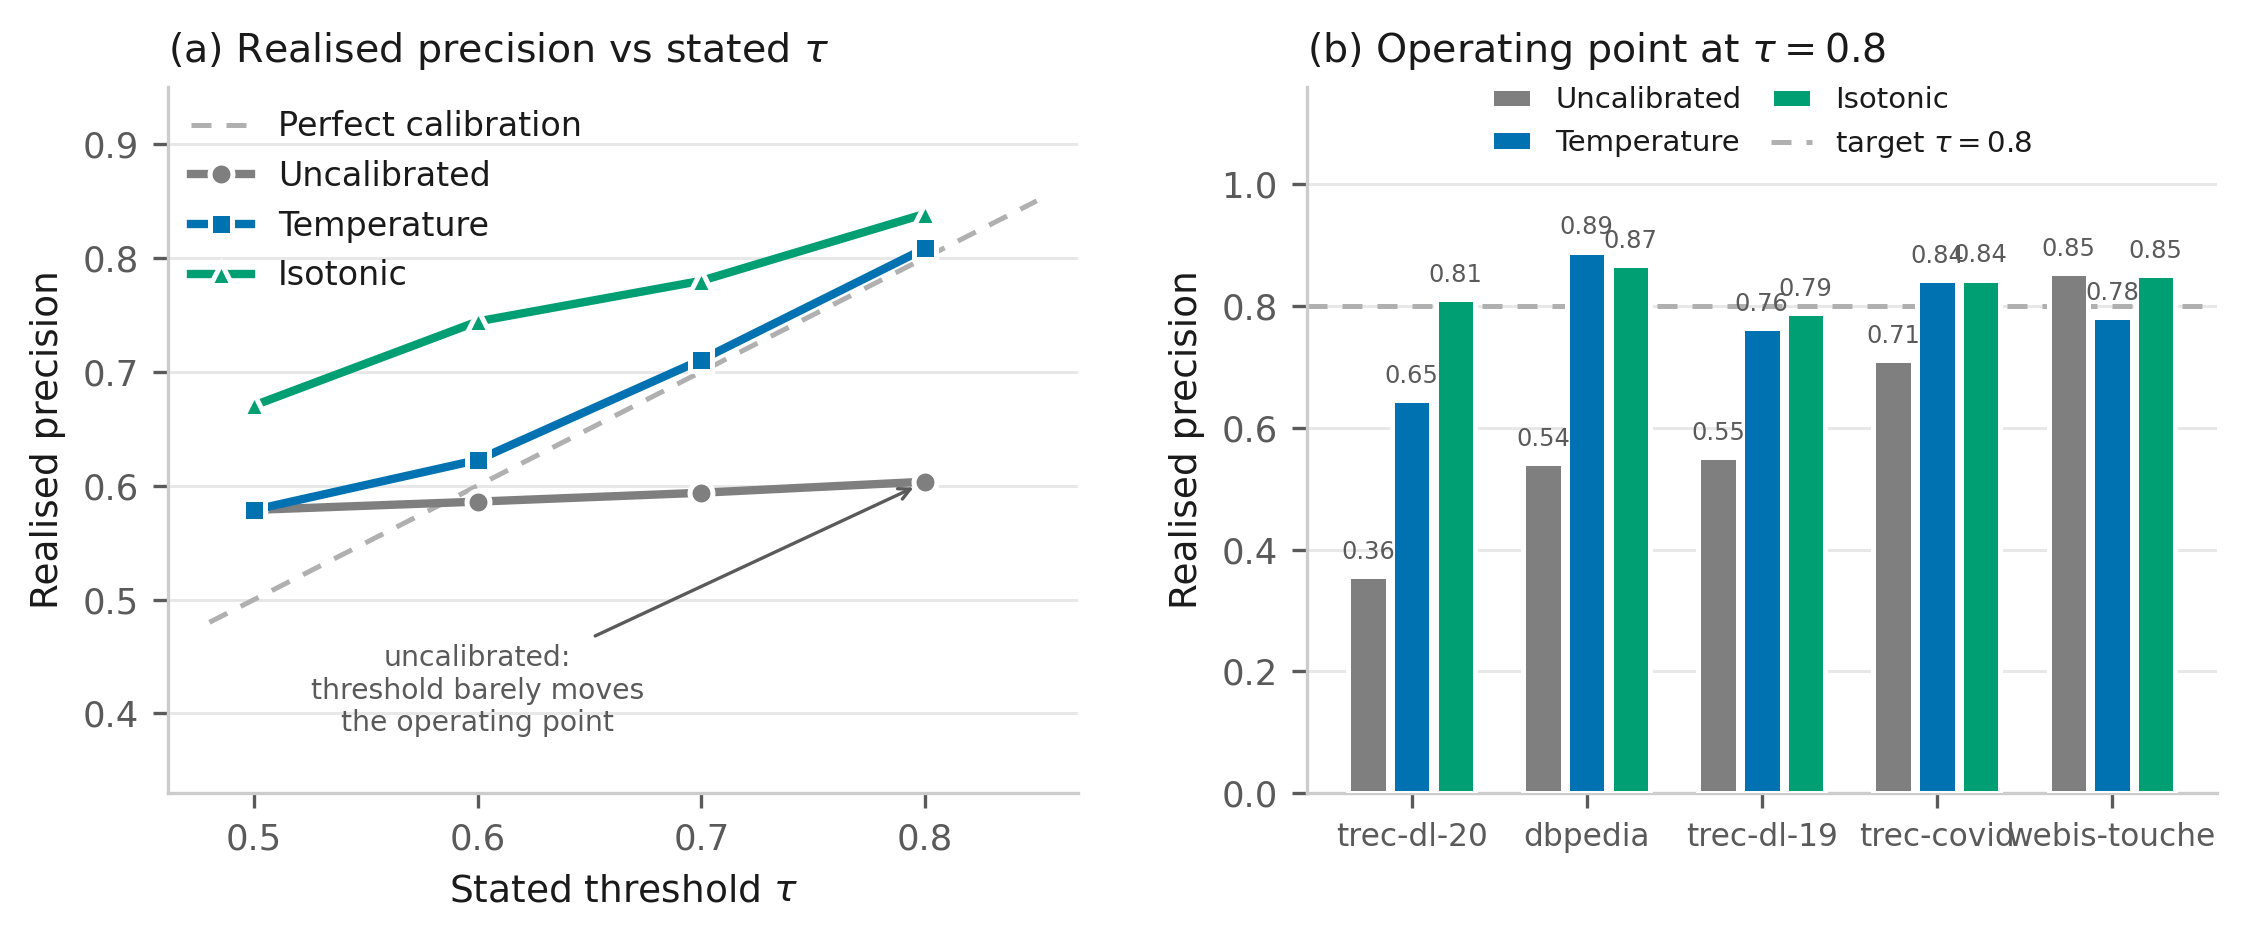
\includegraphics[width=\columnwidth]{paper_fig_threshold_honesty.png}
\Description{Two panels. Left: realised precision versus stated threshold, where the uncalibrated curve is nearly flat. Right: realised precision at a threshold of 0.8 by collection, where calibration sharply reduces the cross-collection spread.}
\caption{(a) Raising $\tau$ barely moves the uncalibrated operating point. (b) At
$\tau{=}0.8$ the uncalibrated realised precision varies widely across collections;
after calibration it does not.}\label{fig:honesty}
\end{figure}

\subsection{A worked example}\label{sec:casestudy}
It is worth seeing what the aggregate precision gain of the previous subsection looks
like on individual pairs. Consider MiniLM-L6, a default re-ranker in several RAG
toolkits, on the held-out half of TREC~DL~2019 at $\tau = 0.8$. The raw scores accept
$1{,}108$ passages at that cut with a precision of only $0.52$; after isotonic
calibration the accepted set shrinks to $220$ passages with a precision of $0.79$. The
mechanism is visible in the individual demotions: the raw model assigns probability
$1.00$ to many passages that the assessors did not judge relevant, and calibration
reduces that unwarranted certainty to about $0.77$, just below the threshold.
Table~\ref{tab:cases} shows three such passages, each topically plausible but a
near-miss rather than an answer. Of all passages the raw score accepted and
calibration then rejected, $55\%$ were genuinely non-relevant; the remainder are
relevant passages demoted along with them, which is the coverage cost noted above and
is expected given that monotone calibration cannot improve the precision--coverage
frontier, only relocate the operating point onto it.

\begin{table}[t]
\centering
\caption{Three held-out passages (MiniLM-L6, TREC~DL~2019) that the raw score accepts
with full confidence at $\tau{=}0.8$ but that the assessors did not judge relevant.
Calibration lowers the probability below the threshold, rejecting them.}
\label{tab:cases}
\small
\renewcommand{\arraystretch}{1.15}
\begin{tabular}{p{0.60\columnwidth}rr}
\toprule
\thead{Query / passage (truncated)} & \thead{$p_{\text{raw}}$} & \thead{$p_{\text{iso}}$} \\
\midrule
\emph{q:} causes of left ventricular hypertrophy \newline
\emph{d:} ``Ventricular hypertrophy is thickening of the walls of a ventricle of the
heart\ldots'' & 1.00 & 0.77 \\
\midrule
\emph{q:} example of monotonic function \newline
\emph{d:} ``To solidify our understanding of what a monotonic function is, let's
consider a non-monotonic\ldots'' & 1.00 & 0.77 \\
\midrule
\emph{q:} is CDG airport in main Paris \newline
\emph{d:} ``You can take the RER Line~B suburban train from Paris-Charles de Gaulle
(CDG) Airport to central\ldots'' & 1.00 & 0.77 \\
\bottomrule
\end{tabular}
\end{table}

\subsection{The improvement is stable}\label{sec:robust}
The conclusions are properties of the models, not artifacts of the measurement. ECE
is binning-dependent in general, so we recomputed every value under ten schemes
(equal-width and equal-mass binning at $5$, $10$, $15$, $20$, and $30$ bins): the mean
ECE varies by under $0.004$, the per-pair spread across all ten schemes averages
$0.004$, and the model ranking is identical under nine of the ten. The temperature
search cap likewise does not affect the valid subset: relaxing it moves mean ECE by
only $0.005$, and the few divergent optima all fall on collections the diagnostic
already excludes, where divergence is the expected signature of a positive-only
judged set.

The validity diagnostic of Equation~(2) is itself robust to its two thresholds. We
swept the minority-support floor over $\{50, 100, 150\}$ and the prevalence ceiling
over $\{0.85, 0.90, 0.95\}$, a full $3\times3$ grid, and re-classified all eleven
collections. Nine of the eleven receive the same verdict under every setting: the four
balanced collections are always valid and the five positive-only collections always
invalid. Only two borderline collections move, and both in the expected direction ---
scidocs becomes valid only under the most permissive corner ($K{=}50$, $\pi\le0.95$),
and webis-touche2020, with $140$ negatives, drops out only when the floor is raised to
$150$. The default $(100, 0.90)$ yields five valid collections and sits in the stable
interior of the grid. Table~\ref{tab:full} reports the complete per-pair results
underlying the aggregates above, so that every number can be inspected directly.

\begin{table*}[t]
\centering
\caption{Complete per-pair results on the valid subset (five main models $\times$
five collections, held-out split). Every method improves on the raw baseline in every
one of the twenty-five pairs. Temperature's advantage is largest where prevalence is
lowest; Platt and isotonic are strong throughout.}\label{tab:full}
\small
\begin{tabular}{llrrrrrr}
\toprule
\thead{Model} & \thead{Collection} & \thead{Prev.} & \thead{raw ECE} & \thead{$T$} & \thead{temp ECE} & \thead{Platt ECE} & \thead{iso ECE} \\
\midrule
TinyBERT-L2 & trec-dl-20 & 0.17 & 0.395 & 10.69 & 0.343 & 0.029 & 0.018 \\
            & dbpedia    & 0.35 & 0.281 &  6.75 & 0.196 & 0.030 & 0.024 \\
            & trec-dl-19 & 0.35 & 0.325 &  8.45 & 0.173 & 0.046 & 0.045 \\
            & trec-covid & 0.62 & 0.276 &  6.48 & 0.055 & 0.057 & 0.033 \\
            & webis-touche & 0.78 & 0.339 & 11.08 & 0.244 & 0.060 & 0.032 \\
\midrule
MiniLM-L6   & trec-dl-20 & 0.17 & 0.401 &  9.60 & 0.349 & 0.017 & 0.015 \\
            & dbpedia    & 0.35 & 0.297 &  5.83 & 0.219 & 0.027 & 0.023 \\
            & trec-dl-19 & 0.35 & 0.312 &  6.56 & 0.180 & 0.046 & 0.037 \\
            & trec-covid & 0.62 & 0.235 &  4.40 & 0.045 & 0.044 & 0.027 \\
            & webis-touche & 0.78 & 0.229 &  4.83 & 0.215 & 0.103 & 0.050 \\
\midrule
MiniLM-L12  & trec-dl-20 & 0.17 & 0.422 & 11.67 & 0.351 & 0.021 & 0.013 \\
            & dbpedia    & 0.35 & 0.313 &  6.59 & 0.221 & 0.028 & 0.019 \\
            & trec-dl-19 & 0.35 & 0.329 &  7.14 & 0.194 & 0.059 & 0.035 \\
            & trec-covid & 0.62 & 0.251 &  4.84 & 0.058 & 0.044 & 0.042 \\
            & webis-touche & 0.78 & 0.166 &  3.97 & 0.160 & 0.110 & 0.038 \\
\midrule
ELECTRA-base& trec-dl-20 & 0.17 & 0.139 &  2.84 & 0.087 & 0.019 & 0.016 \\
            & dbpedia    & 0.35 & 0.330 &  6.84 & 0.164 & 0.035 & 0.021 \\
            & trec-dl-19 & 0.35 & 0.250 &  5.92 & 0.035 & 0.036 & 0.038 \\
            & trec-covid & 0.62 & 0.285 &  4.77 & 0.084 & 0.084 & 0.025 \\
            & webis-touche & 0.78 & 0.283 &  6.10 & 0.249 & 0.068 & 0.052 \\
\midrule
BGE-base    & trec-dl-20 & 0.17 & 0.262 &  3.37 & 0.286 & 0.020 & 0.018 \\
            & dbpedia    & 0.35 & 0.159 &  2.96 & 0.107 & 0.028 & 0.022 \\
            & trec-dl-19 & 0.35 & 0.207 &  3.29 & 0.145 & 0.031 & 0.039 \\
            & trec-covid & 0.62 & 0.228 &  4.39 & 0.037 & 0.041 & 0.028 \\
            & webis-touche & 0.78 & 0.292 &  6.78 & 0.236 & 0.068 & 0.019 \\
\bottomrule
\end{tabular}
\end{table*}

% =============================================================================
\section{Limitations}\label{sec:limitations}

Three limitations bound the scope of these findings. First, all seven re-rankers are
encoder-based cross-encoders; we do not evaluate generative or LLM-based re-rankers
such as RankLLaMA~\cite{ma2024rankllama}, which score relevance through a language
model's output distribution and may exhibit a different calibration profile. The
hazard and diagnostic of Sections~\ref{sec:hazard}--\ref{sec:diagnostic} concern the
evaluation data and so apply regardless of the scoring model, but the specific
magnitudes and the method ordering are established only for the encoder family.
Second, our deeply pooled collections are the TREC Deep Learning 2019 and 2020 passage
tracks; extending to later tracks (2021--2022, over MS~MARCO~v2) would further widen
the valid subset and is a natural next step, though the five collections here already
span prevalences from $0.17$ to $0.78$. Third, the study is English-language, and one
valid collection, webis-touche2020, is both small ($49$ queries) and the case on which
several conclusions are weakest, being where models are under-confident and where
transferred Platt scaling fails; the two collections that most firmly support the
results are dbpedia-entity and the TREC~DL tracks. The diagnostic thresholds are
conventional rather than derived, but the sweep in Section~\ref{sec:robust} shows the
resulting classification is stable around them.

% =============================================================================
\section{Conclusion}\label{sec:conclusion}

Cross-encoder re-rankers are overconfident, and their scores should not be consumed as
probabilities without correction. The sharper lesson is methodological: most standard
retrieval collections cannot measure calibration, because their judged sets lack
negatives, and the naive analysis on such data is not merely noisy but inverted.
Reporting qrel prevalence and applying the validity diagnostic before trusting any
calibration figure is a cheap and necessary safeguard, and adopting deeply pooled
collections such as the TREC~DL tracks makes valid measurement possible. Where
measurement is valid, calibration is effective, free of ranking cost, and portable
across domains as a per-model temperature; it converges different re-rankers to
comparable calibration; and its concrete payoff is a threshold that means what it
says. We release the scored pairs, fitted calibrators, and code so that cross-domain
calibration evaluation in IR becomes routine rather than accidental.

\balance
\bibliographystyle{ACM-Reference-Format}
\bibliography{calrank}

\end{document}
